% Shared by main.tex and report.tex; numerical tables are generated from executed runs.
\subsection{Experiment Design and Error Definitions}\label{sec:nav-experiments}

The navigation campaign was executed on 10 November 2026 using
\path{report_assets/generate_navigation.py}, with the physically sampled ESKF and
seed~0 for the paired comparisons, supplemented by the multi-seed experiments below. It supplements the earlier physics campaign. Two paired closed-loop tests use
\path{project2_landing} and \path{flight_calibrated_landing}. Within each pair,
the resolved configuration is identical except for the navigation module; the generation
script checks that invariant. Initial-state dispersion is disabled. Each run propagates
its own closed-loop trajectory, so the comparison measures the effect of navigation on
the combined estimation, planning, and control response.

The Project~2 pair starts at 300 m and 25 m/s downward speed, with ideal actuators and a
free-terminal-time LCvx plan. The calibrated pair starts at 348.764 m and 76.111 m/s
downward speed, with mass 35,692.161 kg, realistic actuators, and the scenario's previously
selected aerodynamic parameters. Its LCvx plan uses a 12.145 s terminal time, a 30 kN/s
planned thrust-rate limit, and vertical tracking gains of 6 s$^{-2}$ and 4 s$^{-1}$.
These settings originate from the separate flight-calibration study; no parameters are
refitted to the sensor samples. Neither differences between these two scenario families
nor the calibrated scenario's fit to public observables are treated as navigation errors.
Both use a 1 ms plant step, 10 ms navigation period, and 20 ms control period. The guidance
interface is called every second, but \texttt{convex\_replan=false} retains the initial plan
while tracking feedback continues. Trajectory logging periods remain 100 ms and 20 ms,
respectively; all navigation errors use the full 10 ms navigation grid.

For vector state $\bm x$, error magnitude and reported summary statistics are
\begin{equation}
 e_k=\|\widehat{\bm x}_k-\bm x_{truth,k}\|_2,\qquad
 \mathrm{RMSE}=\sqrt{\frac1N\sum_{k=1}^{N}e_k^2},\qquad e_{\max}=\max_k e_k.
\end{equation}
Attitude error is the shortest relative-quaternion rotation angle, reported in degrees;
angular-rate error is the norm of the body/reference rate difference, reported in degrees
per second. Initialization transients are included. Navigation samples stop at the last
scheduled update before the plant terminates. Ground-contact speed, miss distance, and
tilt use the simulator's interpolation to zero radial altitude; contact time in the tables
is interpolated with the same logged-state bracket. These terminal quantities and the
navigation samples are therefore evaluated at distinct epochs.

\subsection{Closed-Loop Navigation and Landing Results}\label{sec:nav-closed-loop}

All four nominal cases reach a soft landing under the existing simulator criteria.
Table~\ref{tab:nav-contact} compares the paired terminal results and
Table~\ref{tab:nav-errors} reports ESKF accuracy against each run's own truth.
Identity navigation has exactly zero estimation error because it returns truth.
It is an ideal-feedback reference, not an unfiltered sensor estimator.

\begin{table}[!htbp]\centering\small
\caption{Paired closed-loop results, seed 0. Each pair changes only navigation.
All four cases satisfy the simulator's soft-landing and success criteria.}\label{tab:nav-contact}
% Generated by report_assets/generate_navigation.py; do not edit numbers.
\begin{tabularx}{\textwidth}{ll*{4}{>{\raggedleft\arraybackslash}X}}\toprule
Scenario & Navigation & Contact [s] & Speed [m/s] & Miss [m] & Tilt [deg]\\\midrule
Project 2 & Identity & 17.468 & 0.086 & 0.019 & 0.055\\
Project 2 & ESKF & 17.583 & 1.381 & 0.788 & 0.219\\
Calibrated & Identity & 12.230 & 0.483 & 0.014 & 0.062\\
Calibrated & ESKF & 12.195 & 0.553 & 0.602 & 1.097\\
\bottomrule\end{tabularx}

\end{table}

\begin{table}[!htbp]\centering\small
\caption{ESKF navigation error statistics on the full navigation grid. Vector entries use
norms, not componentwise averages.}\label{tab:nav-errors}
\begin{tabularx}{\textwidth}{ll*{4}{>{\raggedleft\arraybackslash}X}}\toprule
Scenario & Statistic & Position [m] & Velocity [m/s] & Attitude [deg] & Rate [deg/s]\\\midrule
Project 2 & RMSE & 0.540 & 0.066 & 1.356 & 0.048\\
Project 2 & MAX & 2.879 & 0.182 & 2.444 & 0.131\\
Calibrated & RMSE & 0.641 & 0.074 & 1.189 & 0.049\\
Calibrated & MAX & 2.879 & 0.166 & 2.282 & 0.125\\
\bottomrule\end{tabularx}

\end{table}
\FloatBarrier

The ESKF introduces observable feedback consequences. In the Project~2 pair, contact speed
increases from 0.086 to 1.381 m/s while the position-estimation RMSE is 0.540 m. In the
calibrated pair, contact speed changes from 0.483 to 0.553 m/s and horizontal miss increases
from 0.014 to 0.602 m, with position-estimation RMSE 0.641 m. Thus sub-metre average
estimation error does not imply unchanged terminal performance. The plots show estimation
transients and the resulting trajectories; they do not establish robustness probabilities
from a single noise realization.

\begin{figure}[!htbp]\centering
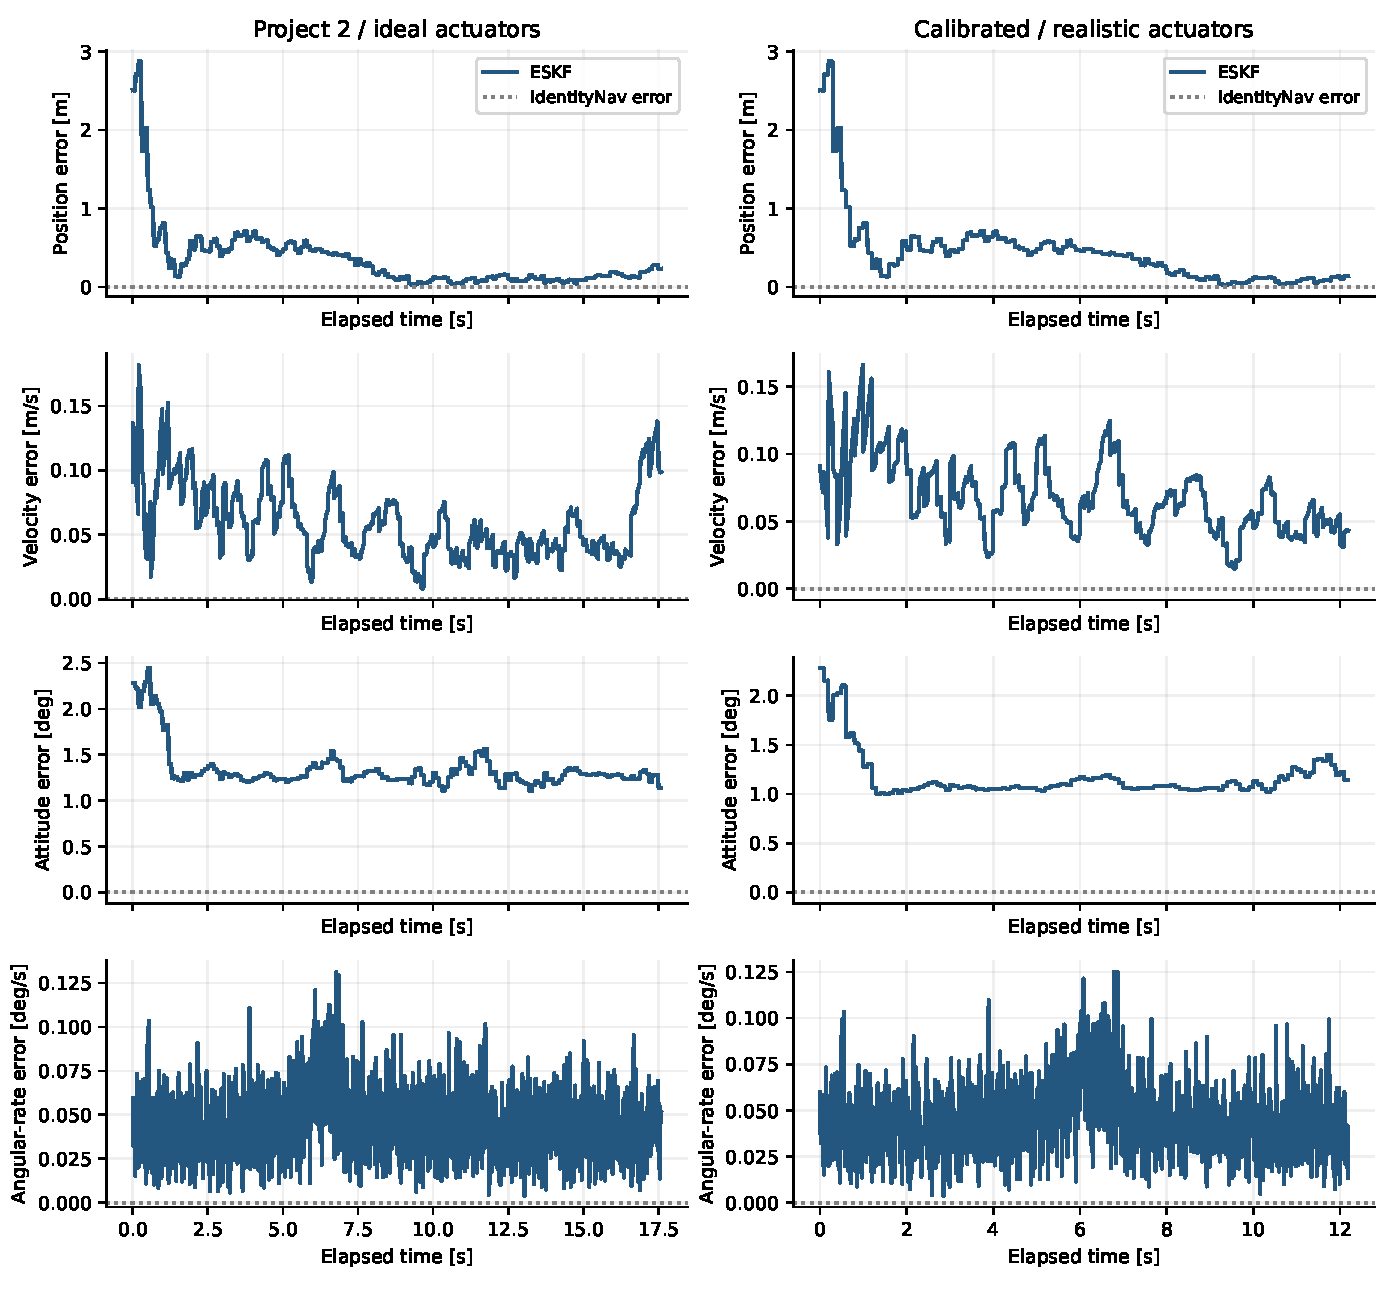
\includegraphics[width=\textwidth,height=0.72\textheight,keepaspectratio]{report_assets/navigation_closed_loop.pdf}
\caption{ESKF position, velocity, attitude, and angular-rate error norms in the two
closed-loop cases. Dotted zero lines indicate ideal-feedback estimation error.
Each ESKF history is compared with its own plant truth.}\label{fig:nav-closed-loop}
\end{figure}

\begin{figure}[!htbp]\centering
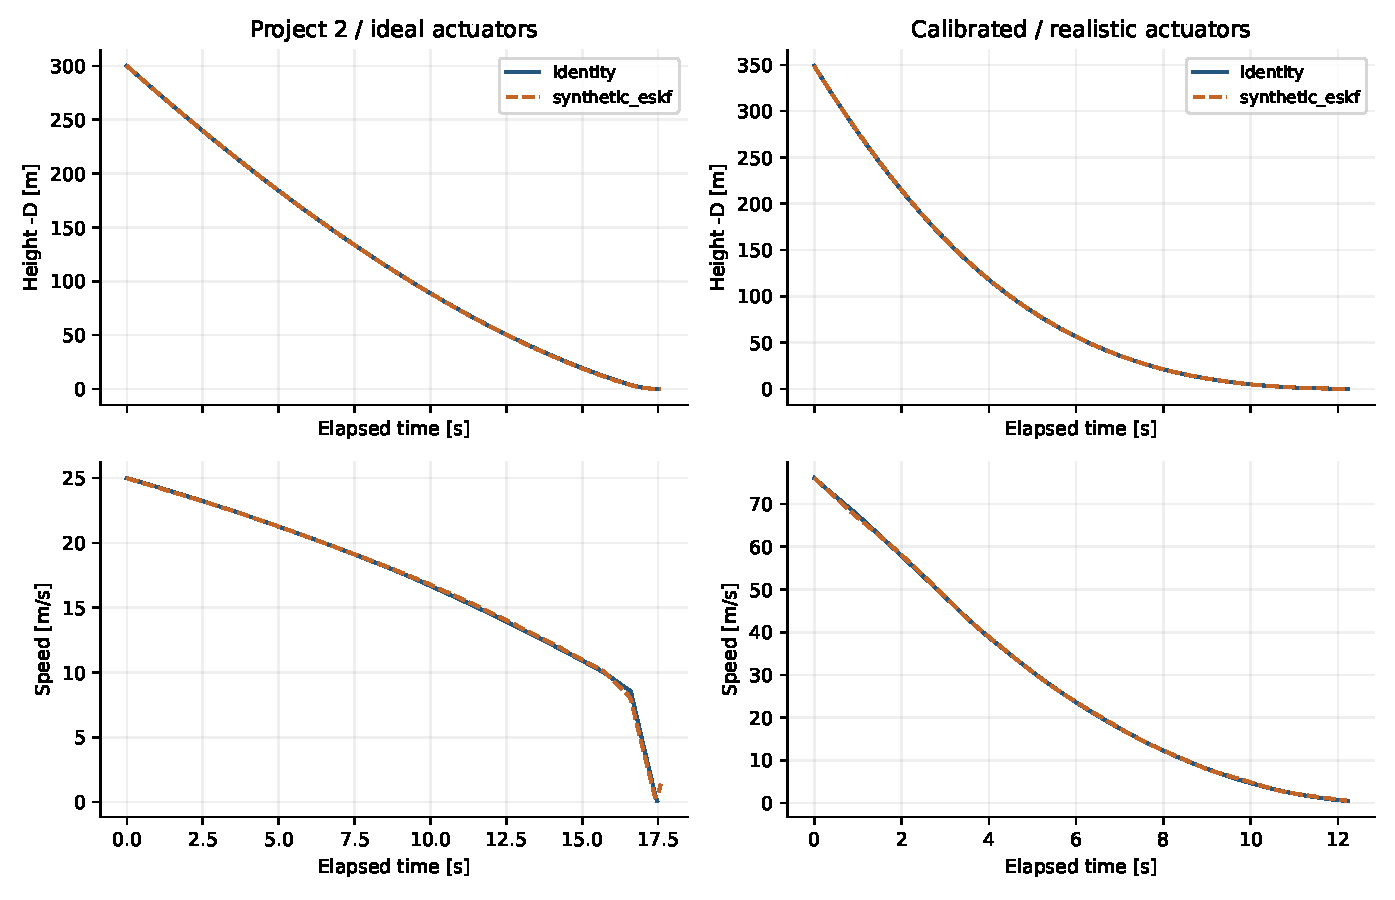
\includegraphics[width=\textwidth,height=0.58\textheight,keepaspectratio]{report_assets/navigation_landing.pdf}
\caption{True height and speed under identity and ESKF feedback. The height curves use
the near-pad tangent height $-r_D$; contact metrics use radial altitude.
Each panel retains its scenario's plant and controller settings.}\label{fig:nav-landing}
\end{figure}

\subsection{Fixed-Trajectory Filter Comparison and GNSS Outage}\label{sec:nav-replay}

To isolate estimation from changing closed-loop trajectories, the calibrated identity
run's truth is replayed at 100 Hz. Native CG force and inertial-rate histories are recorded at every navigation epoch.
One sensor generator uses these histories to create a common sample sequence; each filter receives an independent copy of the same measurements. Three cases
share the same GNSS/radar initialization and uncertain alignment observation: IMU-only propagation
with all subsequent aiding disabled, the nominal ESKF, and an ESKF with GNSS updates
suppressed from 4 through 8 s while radar remains available. The replay has 1,223 IMU
samples over 0--12.22 s, 121 valid nominal GNSS updates, and 245 radar samples. Suppressing
the selected interval leaves 80 GNSS updates. No replay estimate is fed back into the plant.

\begin{table}[!htbp]\centering\small
\caption{RMSE on identical truth and sensor samples. The IMU-only case retains the common
initial aided update and then propagates without further GNSS or radar corrections.}
\label{tab:nav-replay}
\begin{tabularx}{\textwidth}{l*{4}{>{\raggedleft\arraybackslash}X}}\toprule
Replay case & Position [m] & Velocity [m/s] & Attitude [deg] & Rate [deg/s]\\\midrule
IMU only & 19.732 & 4.307 & 2.318 & 0.044\\
ESKF & 0.641 & 0.075 & 1.091 & 0.049\\
ESKF + GNSS outage & 0.756 & 0.068 & 1.114 & 0.045\\
\bottomrule\end{tabularx}

\end{table}
\FloatBarrier

GNSS/radar aiding reduces position RMSE from 19.732 to 0.641 m and velocity RMSE from
4.307 to 0.075 m/s. A four-second GNSS outage increases position RMSE to 0.756 m; radar
continues to constrain height. The slight decrease in aggregate velocity RMSE during this
particular outage is not evidence that discarding GNSS is beneficial. It is one finite
noise realization, and the horizontal and vertical channels have different aiding.

With uncertain initial alignment, attitude RMSE decreases from 2.318 deg in IMU-only
propagation to 1.091 deg with ESKF aiding. Angular-rate RMSE is 0.044 deg/s and
0.049 deg/s, respectively: aiding does not reduce every error metric. The short,
nearly vertical trajectory has no direct attitude observation after initialization.
Figure~\ref{fig:nav-biases} shows that not every bias component converges; the longer
ascent and consistency experiments below examine a wider excitation and time range.

\begin{figure}[!htbp]\centering
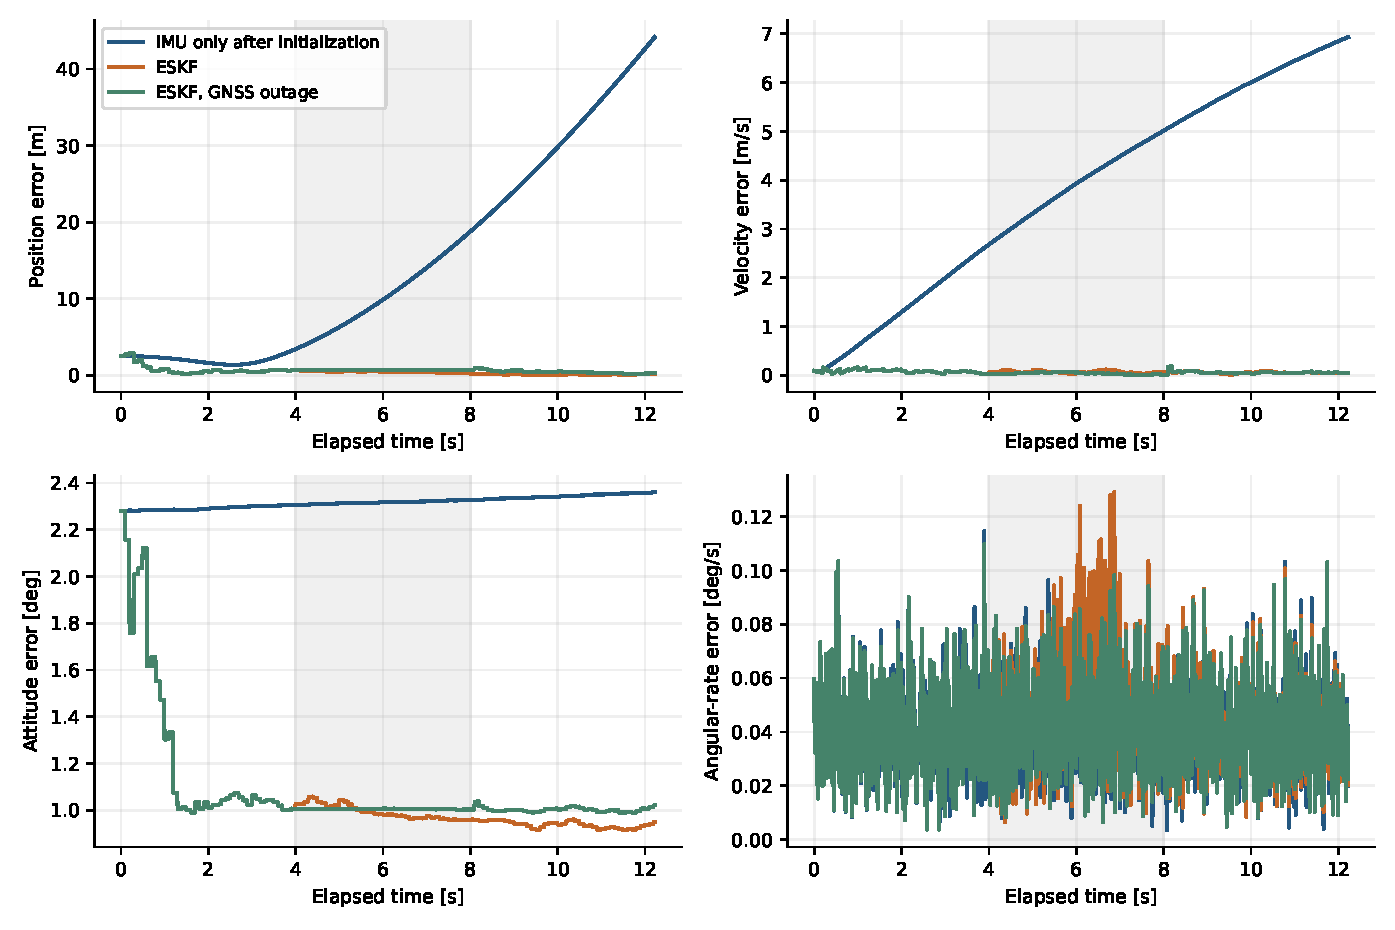
\includegraphics[width=\textwidth,height=0.60\textheight,keepaspectratio]{report_assets/navigation_replay.pdf}
\caption{Fixed-truth replay comparison. The shaded interval is the GNSS outage applied
only to the outage variant; radar remains active. All three cases receive the same IMU
samples and start from the same nominal state and covariance.}\label{fig:nav-replay}
\end{figure}

\begin{figure}[!htbp]\centering
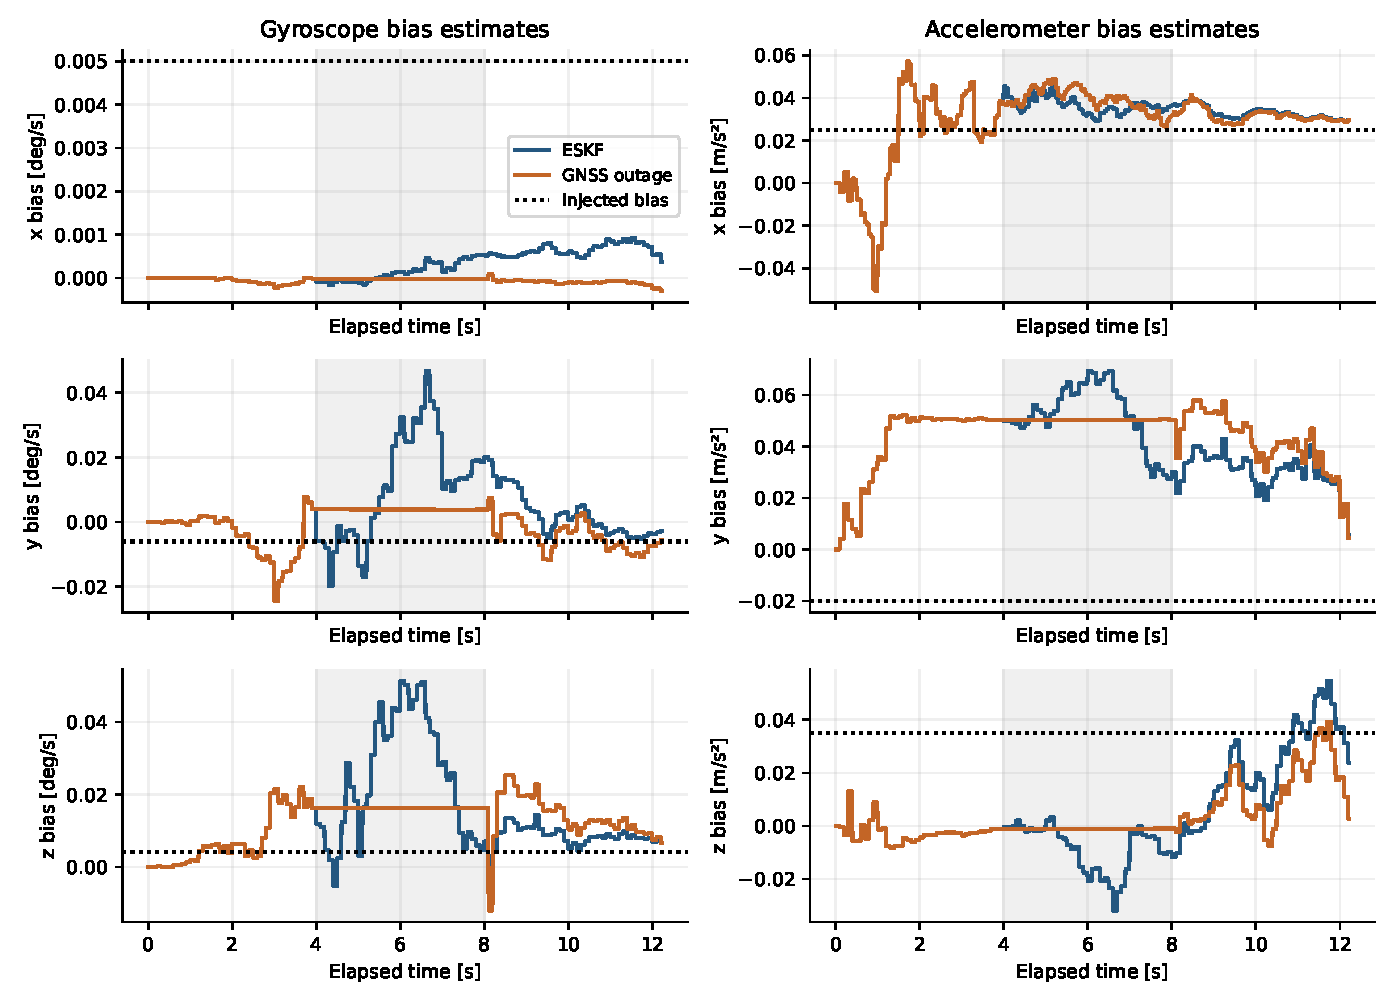
\includegraphics[width=\textwidth,height=0.63\textheight,keepaspectratio]{report_assets/navigation_biases.pdf}
\caption{Estimated IMU biases in fixed-truth replay, with the constant injected biases
shown as dotted lines. The short experiment does not show convergence of every bias
component. The shaded interval suppresses GNSS only in the outage variant.}\label{fig:nav-biases}
\end{figure}

\FloatBarrier
\subsection{Multiple Seeds and Missing-GNSS Startup}\label{sec:nav-robustness}
Each landing scenario is repeated with seeds 0--9, a 1 deg per-axis initial alignment
uncertainty, and the same sensor parameters and unchanged controller settings. A third
condition uses the Project~2 landing with GNSS suppressed from 0 through 3 s. Its declared
initial position prior has offset $(10,-8,5)$ m and velocity prior has offset
$(0.5,-0.4,0.3)$ m/s; radar remains available. Thus the prior is deliberately different
from truth, and the estimator must propagate and acquire GNSS after startup.
\begin{table}[!htbp]\centering\small
\caption{Ten-seed closed-loop evaluation per condition. Maxima include unsuccessful runs;
mean position RMSE is the arithmetic mean of the ten per-run RMSEs.}\label{tab:nav-seeds}
\begin{tabularx}{\textwidth}{Yrrrr}\toprule
Case & Soft success & Max speed [m/s] & Max miss [m] & Mean pos. RMSE [m]\\\midrule
Project 2 & 5/10 & 6.539 & 1.152 & 0.539\\
Calibrated & 10/10 & 1.314 & 1.836 & 0.615\\
Project 2, startup outage & 4/10 & 4.444 & 4.358 & 5.973\\
\bottomrule\end{tabularx}

\end{table}
\FloatBarrier
The calibrated realistic-actuator case succeeds in all ten runs. The original Project~2
configuration succeeds in five; with the startup outage and perturbed prior it succeeds
in four. The nominal Project~2 maximum contact speed is 6.539 m/s despite a mean
position-estimation RMSE of 0.539 m. These outcomes show that the original ideal-actuator
landing configuration is sensitive to state-estimation errors. Successful initialization
and sub-metre average estimation error do not guarantee a soft landing. The empirical
counts describe these finite trials, not a qualified flight success probability; no
controller gains were changed to improve the counts. The two scenario families differ in
initial condition, vehicle and guidance settings, so their success counts do not isolate
the effect of actuator fidelity.

\subsection{Long Ascent Replay and Covariance Diagnostics}\label{sec:nav-consistency}
The native 150-second \texttt{project2\_ascent} trajectory is recorded at 100 Hz,
including its 10--12 s gimbal maneuver, throttle changes, cutoff at 145 s, and coast.
The physical IMU channels come directly from native loads and inertial angular rates.
Five seeds (0--4) are replayed under three conditions: nominal aiding, no GNSS from
0 through 5 s, and no GNSS from 60 through 80 s. The startup case uses the same nonzero
prior offsets as the landing test. All variants within each seed receive identical
sensor samples and alignment observation; only GNSS availability and the startup
initialization differ. Radar follows the 1500 m range limit and cannot aid the
high-altitude 20-second outage. Estimates are not fed back into this prescribed ascent.
\begin{table}[!htbp]\centering\small
\caption{Five-seed 150-second ascent replay. RMSE columns are means of per-run RMSEs;
NEES is averaged over the five seeds and all sampled epochs.}\label{tab:nav-ascent}
\begin{tabularx}{\textwidth}{Yrrrr}\toprule
Ascent case & Pos. RMSE [m] & Vel. RMSE [m/s] & Att. RMSE [deg] & Mean NEES\\\midrule
Nominal & 0.380 & 0.054 & 0.750 & 10.70\\
Startup outage (5 s) & 2.833 & 0.262 & 0.866 & 10.83\\
In-flight outage (20 s) & 1.059 & 0.143 & 0.933 & 11.17\\
\bottomrule\end{tabularx}

\end{table}
\FloatBarrier
All startup-outage runs acquire GNSS at 5.1 s. Initial attitude-error magnitudes range
from 0.703 to 2.332 deg. Across the fifteen ascent replays, final position-error magnitude
is at most 0.414 m and final attitude error at most 0.715 deg. The nominal mean position
RMSE is 0.380 m; the startup and in-flight outages increase it to 2.833 and 1.059 m.
The maximum transient position errors are 23.389 m and 8.664 m in the two outage
conditions. These results demonstrate recovery after aiding returns, rather than
continuous nominal accuracy during the outages.

The full 15-state normalized estimation error squared and measurement normalized
innovation squared are
\begin{equation}
 \mathrm{NEES}_k=\bm e_k^TP_k^{-1}\bm e_k,\qquad
 \mathrm{NIS}_k=\bm y_k^TS_k^{-1}\bm y_k,
\end{equation}
where $\bm e$ includes position, velocity, global attitude error, and both bias errors.
For five independent seeds, the reference pointwise 95\% band for mean NEES is
$[10.588,20.168]$, obtained from a chi-square distribution with 75 degrees of freedom.
Mean GNSS NIS is 5.995--6.007 (six measurement components), and mean altimeter NIS is
0.992--0.997 (one component). However, only 50.4--59.0\% of epochs have ensemble NEES
inside the reference band. Thus measurement innovations have appropriate mean scale
in these tests, while full-state covariance consistency is not established. The fixed
injected biases are not sampled from the complete Gaussian prior, process bias noise
allows variation absent from truth, and temporal samples are correlated. The band is a
diagnostic reference, not a sequence of independent acceptance tests or a reason to
retune covariance until a desired pass fraction is obtained.
\begin{figure}[!htbp]\centering
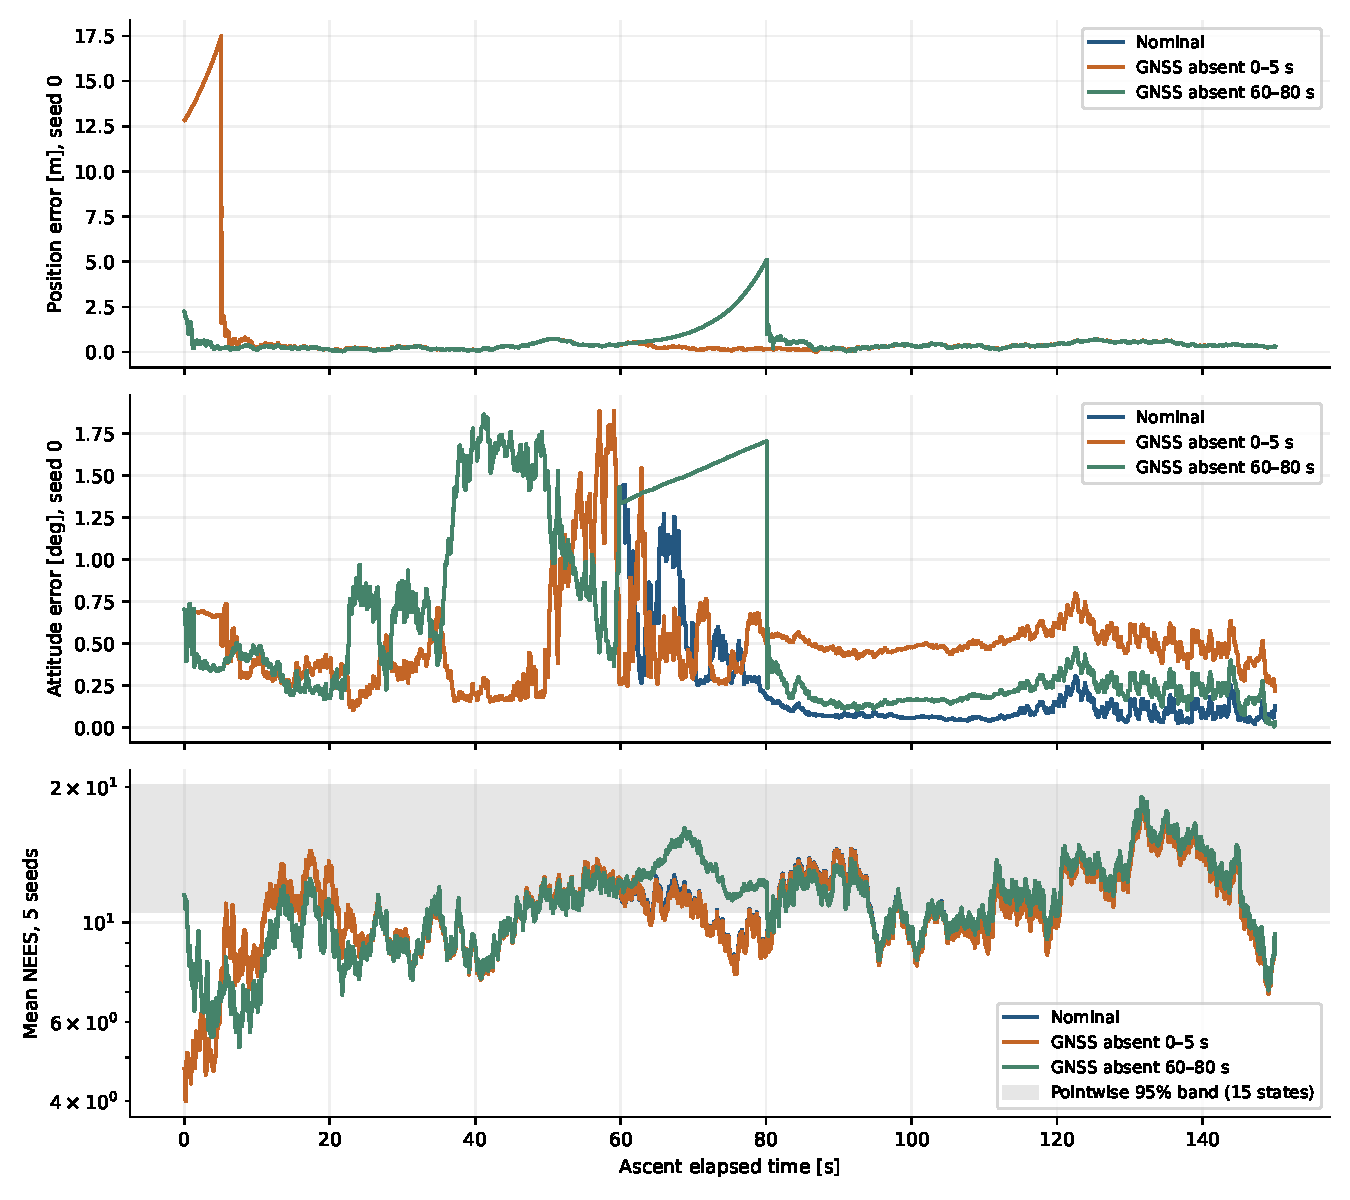
\includegraphics[width=\textwidth,height=0.72\textheight,keepaspectratio]{report_assets/navigation_robustness.pdf}
\caption{Native ascent replay: seed-0 position and attitude error, and five-seed mean NEES.
The pointwise consistency band is shown for the 15-state error.}\label{fig:nav-robustness}
\end{figure}
\FloatBarrier

\subsection{Verification Scope and Remaining Navigation Limitations}\label{sec:nav-limits}
Physical checks cover zero accelerometer output in vacuum free fall, pad support,
Earth-rate gyro output, and drift-free noiseless propagation at an Earth-fixed point
away from the reference origin. Finite differences verify the radial-height/gravity
Jacobians and global attitude reset. Initialization tests exercise absent GNSS,
nonzero alignment error, and single use of the first GNSS sample. Replay checks include
finite estimates, quaternion normalization, and covariance positivity. Additional checks
verify optional scale-factor/random-walk inputs, explicit sensor-rate validation, GNSS
outlier rejection, and common uncertain initialization of the IMU-only and aided estimators.

The expanded study evaluates small unknown alignment errors, delayed GNSS acquisition,
multiple seeds, and longer high-altitude outages. It does not establish autonomous
alignment from an arbitrary unknown attitude, hardware sensor accuracy, global
covariance consistency, or robust landing over the full operating envelope. Mass remains
an ideal auxiliary measurement. The sensors omit latency, lever arms, saturation, and
vibration; the altimeter assumes radial height. These technical limits remain relevant
to guidance and control design even when the filter is numerically well behaved.
